\documentclass[a4paper, 12pt]{extarticle}

\usepackage[french, english]{babel}
\usepackage[utf8]{inputenc}
\usepackage[T1]{fontenc}
\usepackage{graphicx}
\usepackage{multirow}
\usepackage{tikz}

\usepackage{fancyhdr, lastpage}
\pagestyle{fancy}
\fancyfoot[C]{{\thepage}/\pageref{LastPage}}

% \usepackage{fontspec}
% \setmainfont{Times New Roman}
\usepackage{geometry}
\geometry{a4paper,
    total={170mm,257mm},
    left=20mm,
    top=7mm,
 }

% !TeX root = ./kernel/esayRattra.tex

\newcommand{\courseCode}{--}
\newcommand{\courseTitle}{Réseaux intelligents et réseaux industriels}
\newcommand{\examDate}{12 février 2020}
\newcommand{\examType}{RATTRAPAGE}
\newcommand{\teacher}{M. LIEDJI WENKACK Dagobert}
\newcommand{\semester}{1}
\newcommand{\academicYear}{2020-2021}
\newcommand{\timeAllowed}{2 Heures 00 Minutes}
\newcommand{\totalMarks}{20}
\newcommand{\MarksOne}{\scriptsize{(4 points)}}
\newcommand{\MarksTwo}{\scriptsize{(11 points)}}
\newcommand{\MarksThree}{\scriptsize{(5 points)}}
\newcommand{\classLevel}{Master 2 RTS}
\newcommand{\docs}{Aucun}
\begin{document}

\begin{center}
    \begin{tabular}{ccc}
        \textbf{REPUBLIC OF CAMEROON }              & \multirow{7}{*}{\resizebox{3cm}{4cm}{
\includegraphics{../figs/ic_logo.jpg}}} & \textbf{REPUBLIQUE DU CAMEROUN}          \\
        \scriptsize \textbf{PEACE-WORK-FATHERLAND } &                                                                              & \scriptsize \textbf{PAIX-TRAVAIL-PATRIE} \\
        {\small **********}                         &                                                                              & {\small **********}                      \\
        \textbf{UNIVERSITY OF DSCHANG}              &                                                                              & \textbf{UNIVERSITE DE DSCHANG}           \\
        {\small **********}                         &                                                                              & {\small **********}                      \\
        \textbf{FACULTY OF SCIENCE}                 &                                                                              & \textbf{FACULTE DES SCIENCE}             \\
        {\small **********}                         &                                                                              & {\small **********}                      \\
        \textbf{Deparment of physics}               &                                                                              & \textbf{Département de Physique}         \\
    \end{tabular}
\end{center}
% \vspace{0.2cm}
{\centering \rule{\linewidth}{0.03cm}}

\begin{center}
    \textbf{\courseTitle (\courseCode)}\\
    %\textbf{\examType}
\end{center}
\vspace{-0.5cm}
\begin{center}
    \scriptsize
    \begin{tabular*}{\textwidth}{l @{\extracolsep{\fill}} l}
        \textbf{Niveau:} \classLevel & \textbf{Durée:} \timeAllowed\\
        \textbf{Année Académique:} \academicYear & \textbf{Session:} \examType\\
        \textbf{Semestre:} \semester & \textbf{Date:} \examDate\\
        \textbf{Document autorisés:} \docs & \textbf{Enseignant:} \teacher\\
    \end{tabular*}
\end{center}
\vspace{-0.5cm}
{\centering \rule{\textwidth}{0.02cm}}

% !TeX root = ./kernel/esayRattra.tex
% !TeX root = ./kernel/easyExam.tex
\section*{Test de connaissances \MarksOne}
\begin{enumerate}
    \item Définissez les termes suivants:
          \begin{itemize}
              \item Réseaux intélligents
              \item Capteurs, signal, échantillonnage et actionneurs
          \end{itemize}
    \item Donner la signification des protocoles d'échange de données, de et de sécurité des réseaux intélligents suivants:
          \begin{enumerate}
              \item HTTP, M2M, CoAP et MQTT
              \item SSL, TLS et DTLS
          \end{enumerate}
    \item Donner et définissez deux autres protocoles des réseaux intelligents de votre choix.
\end{enumerate}

% !TeX root = ./kernel/esayRattra.tex

% !TeX root = ./kernel/easyExam.tex
\section*{Exercice 2 \MarksThree}
\begin{enumerate}
    \item Donnez trois systèmes d'exploitations utilisés dans la mise en place des réseaux intelligents.
    \item Citez deux (02) outils logiciels et quatre (04) outils matériels utilisés
          dans la mise en place d'un réseaux intelligent.
    \item Citez quatre (04) applications des réseaux intelligents.
    \item Donnez quatre (04) des risques encourus par une organisation ayant un réseaux intelligent mal sécurisé ?
    \item Donnez quatre (04) tâches a éffectuer afin de sécuriser les dispositifs des réseaux intelligents ?
    \item Donner deux (02) avantages des réseaux intelligents.
    \item Identifiez et classifier les cartes de la figure \ref{fig:carte} en carte à microcontrôleurs ou en carte à microprocesseur.
\end{enumerate}

\begin{figure}[!ht]
    \centering
    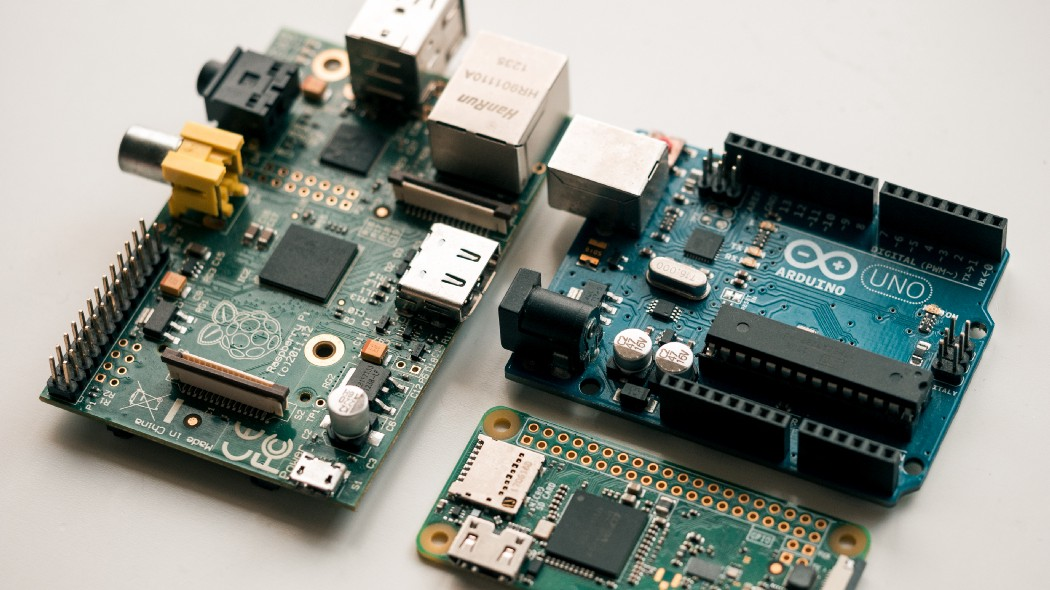
\includegraphics[scale=0.25]{../../figs/hardware_devices.jpg}
    \caption{Quelques cartes pour réseaux intélligents.\label{fig:carte}}
\end{figure}
% !TeX root = ./kernel/easyExam.tex
\section*{Exercice 1 \MarksTwo}

\begin{enumerate}
      \item Décrivez brièvement le fonctionnement d'un réseaux intélligent.
      \item Donner la représentation de l’architecture d’un projet réseau intelligent.
            On insistera uniquement sur les couches principales de l'architecture.
      \item Citez en donnant les fonctions de chaque couches de l'architecture des réseaux intélligents.
      \item Citez 05 (cinq) protocoles des réseaux intélligents.
      \item Quelle est la couche de l'architecture des réseaux intélligents qui interagit directement avec les processus industriels ?
            Comment cette interaction se produit t-elle?
      \item Donnez la différence entre un réseaux dit "non intélligent" et un réseaux intélligent.
\end{enumerate}
La figure \ref{fig:iiot} montre le chef mécanicien vérifiant et contrôlant des robots robots d'automatisation des bras dans l'industrie intelligente d'usine sur le logiciel de système de surveillance en temps réel.

\begin{enumerate}
    \item Donnez trois (03) protocoles réseaux adaptés dans la mise en place de ce réseau intélligent industriel (voir figure \ref{fig:iiot}).
    \item Donnez les élements de chaque couche de l'architecture d'un réseau intélligent se trouvant sur la figure \ref{fig:iiot}.
    \item Donnez deux (02) avantages de ce réseau sur une industrie.
    \item Donnez deux (04) tâches à éffectuer afin d'éviter l'attaque des robots réseau sur les employés de cette l'industrie.
\end{enumerate}

\begin{figure}[!ht]
    \centering
    
\includegraphics[scale=1.4]{../../figs/industrial_inttelings.jpg}
    \caption{Le chef mécanicien vérifie et contrôle des robots robots d'automatisation des bras dans l'industrie intelligente d'usine sur le logiciel de système de surveillance en temps réel.}
    \label{fig:iiot}
\end{figure}


\end{document}